\documentclass[12pt,oneside,a4paper]{book} % This style for A4 format.

\input{./AuxFiles/Packages}

%%%%%%%%%%%%%%%%%%%%%%%%%%%%%%%%%%%%%%%%%%%%%%%%%%%%%%%%%%%%%%%%
%% Document settings
\title{VisuaLearn AI: An Adaptive Multi-Modal Intelligent Learning Platform}
\subCode{IS481P}
% Note: While using the template for IDP, the \Department cmd is not used (discarded automatically) in IDP. The Certificate page uses \guideDeptA[]{} cmd in IDP.
\Department[ISE]{Information Science and Engineering}
\academicYear{2025-26}

%%%%%%%%%%%%%%%%%%%%%%%%%%%%%%%%%%%%%%%%%%%%%%%%%%%%%%%%%%%%%%%%
%% Report Type:
%%%%%%%%%%%%%%%%%% For Plagiarism Check %%%%%%%%%%%%%%%%%%%%%%%
%% Uncomment \EnPlagReport line, before plagiarism check to remove Certificate, Declaration, Acknowledgement and TOC pages.
%\EnPlagReport

%%%%%%%%%%%%%%%%%%% For PG program %%%%%%%%%%%%%%%%%%%
%% Uncomment \pgProgram command and define appropriate values for \MastersIn{} and \pgProgramName{}

%\pgProgram%
\MastersIn[M.Tech]{Master of Technology}
\pgProgramName{VLSI Design \& Embedded Systems}

%%%%%%%%%%%%%%%%%%%%%%%%%%%%%%%%%%%%%%%%%%%%%%%%%%%%%%%%%%%%%%%%
%% Student Details%%%
\stuNameA{Jeevan Raj S B}
\stuUSNA{1RV22IS026}
\stuNameB{R A Nithin Nandana}
\stuUSNB{1RV22IS047}
\stuNameC{Siddesh K R}
\stuUSNC{1RV22IS064}
\stuNameD{Amulya S}
\stuUSND{1RV23IS400}

%%%%%%%%%%%%%%%%%%%%%%%%%%%%%%%%%%%%%%%%%%%%%%%%%%%%%%%%%%%%%%%%
%% Guide Related commands
%% Internal Guide %%
% Have to give both short form and long of Department Name
\guideNameA{Prof. Chethana R}
\guideDesignationA{Assistant Professor}
\guideDeptA[ISE]{Information Science and Engineering}
\guideOrgA{RV College of Engineering}

%% External Guide %%
\guideNameB{Dr. Kavitha S N}
\guideDesignationB{Associate Professor}
\guideDeptB{Dept. of ISE}
\guideOrgB{RV College of Engineering}

%\guideNameC{Dr. Ramavenkateshwaran}
%\guideDesignationC{Assistant Professor}
%\guideDeptC{Dept. of ECE}
%\guideOrgC{RV College of Engineering}

%%%%%%%%%%%%%%%%%%%%%%%%%%%%%%%%%%%%%%%%%%%%%%%%%%%%%%%%%%%%%%%%
%% Esteem members related commands
%% Pannel Members %%
\panelMemberNameA{Dr. Kariyappa}
\panelMemberDesigA{Professor}
\panelMemberDeptA[ISE]{Information Science and Engineering}
\panelMemberNameB{Prof. P N Jayanthi}
\panelMemberDesigB{Assistant Professor}
\panelMemberDeptB[ISE]{Information Science and Engineering}

% Added Ver 3.6 & 3.9
%% Project co-ordinators 
\projectCoOrdNameA{Dr. Vanishree K}
\projectCoOrdDesigA{Associate Professor}
\projectCoOrdDeptA[ISE]{Information Science and Engineering}
% Not used for IDP and Internship
\projectCoOrdNameB{Dr. P N Jayanthi}
\projectCoOrdDesigB{Assistant Professor}
\projectCoOrdDeptB[ISE]{Information Science and Engineering}
%\projectCoOrdNameC{Prof. Subramanya K N}
%\projectCoOrdDesigC{Assistant Professor}

%%%%%%%%%%%%%%%%% Esteemed Members %%%%%%%%%%%%%%%%%%
\HOD{Dr.G.S. Mamatha}
\Principal{Dr. K.N. Subramanya}
% For IDP only
\DeanAcademics{Dr. M.V. Renukadevi}
\VicePrincipal{Dr. K.S Geetha}
%%%%%%%%%%%%%%%%%%%%%%%%%%%%%%%%%%%%%%%%%%%%%%%%%%%%%%%%%%%%%%%%
%%%%%%%%%%%%%%%%%%%%%  QRL %%%%%%%%%%%%%%%%%%%%%%%%%%
\QRurl{https://drive.google.com/drive/folders/1yVk9iKeDNJLtrsY7Gcix4j6q9uOHm-qP?usp=sharing}
%\QRurl{https://drive.google.com/open?id=1jm-POmuq-ZZ1tT5m-xAdCDRnwvLZH8q-}

%%%%%%%%%%%%%%%%%%Draft report%%%%%%%%%%%%%%%%%%
%\DraftCopy %Not yet implemented, if anyone interested, do contact me at pnarashimaraja@rvce.edu.in (or) narashimaraja@gmail.com
%%%%%%%%%%%%%%%%%%%%%%%%%%%%%%%%%%%%%%%%%%%%%%

%%%%%%%%%%%%%%%%%% Glossaries & Acronyms %%%%%%%%%%%%%%%%%%
\newglossary[sym]{symbolList}{sym1}{sym2}{List of Symbols}
\makeglossaries
% Acronyms
\loadglsentries{./AuxFiles/Glossaries}
\renewcommand{\glspostdescription}{}% To remove dot at the end
%%%%%%%%%%%%%%%%%%%%%%%%%%%%%%%%%%%%%%%%%%%%%%

%%%%%%%%%%%%%%%% Bibliography %%%%%%%%%%%%%%%%%%%%%
\usepackage[backend=bibtex,style=ieee]{biblatex}
% If backend is set to bibtex, then configure texmaker Bi(La)Tex with "bibtex %"
\addbibresource{./AuxFiles/ProjectBib.bib}%Add bib file with extention
%%%%%%%%%%%%%%%%%%%%%%%%%%%%%%%%%%%%%%%%%%%%%%

%%%%%%%%%%%%%%%%WaterMark%%%%%%%%%%%%%%%%%%%%%
%% Use it only after Biblatex
%% Uncomment the following lines for watermarking and run it more than 2 times for proper alignment
\usepackage{background}
\backgroundsetup{scale=1, angle=0, firstpage = false, opacity=0.5, position=current page.center, hshift=0pt, vshift=0pt, contents={
\includegraphics[width=0.42\paperwidth]{Figures/RVlogoVecW}}}

\begin{document}
	\NoBgThispage% Don't remove this command, even if you want logo on the first page.	
	\maketitle
	%\pagestyle{empty}
	\newpage
	\ifDrf
	% Remove Certificate, Declaration, Acknowledgement and TOC
	\else
	\begin{spacing}{1.5}
		\input{./CoverPages/Certificate}
		
		\newpage
		\input{./CoverPages/Declaration}
		
		\newpage
		%%ecproject package is created by P Narashimaraja, Assistant Professor, ECE, RVCE.
%%Border
\begin{tikzpicture}[remember picture, overlay]
	\draw[line width = 4pt] ($(current page.north west) + (0.75in,-0.75in)$) rectangle ($(current page.south east) + (-0.75in,0.75in)$);
\end{tikzpicture}
\thispagestyle{empty}
\begin{center}
	\Large\textbf{\underline{ACKNOWLEDGEMENTS}} \par
\end{center}

We are deeply indebted to our internal guide, \textbf{\printGuideNameA}, \printGuideDesigA, Department of \printGuideDeptAInSF, RVCE, for the wholehearted support, suggestions, and valuable advice throughout our project work and for guiding us in the preparation of this report.\\ \par

We express our sincere gratitude to our external guide, \textbf{\printGuideNameB}, \printGuideDesigB, Dept. of ISE, \printGuideOrgB, for her guidance, technical inputs, and encouragement during the development of VisuaLearn AI.\\ \par

Our sincere thanks to the project coordinator, \textbf{\printProjectMemberA}, \printProjectMemberDesigA, Department of \printProjectMemberDeptAInSF, for the timely instructions and support in coordinating the project.\\ \par

We are grateful to \textbf{\printHOD}, Professor and Head, Department of \printDepartmentLF, RVCE, for the support and encouragement.\\ \par

We express sincere gratitude to \textbf{\printVicePrincipal}, Vice-Principal, RVCE, and \textbf{\printPrincipal}, Principal, RVCE, for providing the academic environment and institutional support required to complete this project successfully.\\ \par

We thank all the teaching staff and technical staff of the Department of \printDepartmentLF, RVCE, for their help. Lastly, we thank our family members and friends who provided constant support throughout the project work.\\ \par

		
		\newpage
		\pagenumbering{roman}
		
		\chapter*{Abstract}
		\addcontentsline{toc}{chapter}{Abstract}\vspace{-1cm}
%Border
\begin{tikzpicture}[remember picture, overlay]
  \draw[line width = 4pt] ($(current page.north west) + (0.75in,-0.75in)$) rectangle ($(current page.south east) + (-0.75in,0.75in)$);
\end{tikzpicture}

\noindent VisuaLearn AI is an adaptive multi-modal intelligent learning platform designed to improve conceptual understanding through structured explanations, interactive visualizations, algorithm simulations, quizzes, flashcards, mind maps, voice interaction, and personalized learning flows. Conventional learning tools often present static text or video content and leave the learner to decide how to study, revise, and practise. This project addresses that gap by organizing generated learning material into reusable artifacts and by selecting suitable teaching strategies based on learner context.

The system follows a modular full-stack architecture. The frontend provides a responsive learning workspace with chat, learning tabs, simulation viewers, visual widgets, persona settings, and voice controls. The backend coordinates request routing, authentication, session handling, learning content generation, simulation detection, visualization handling, feedback collection, and persistence. Conversations and learning resources are stored so that learners can revisit previous sessions and continue revision without regenerating every resource.

The major contribution of this project is the integration of multiple educational modes into a single adaptive workflow. A learner can ask a question, receive a structured explanation, open flashcards, attempt a quiz, inspect a mind map, or run a simulation where the topic supports procedural learning. The adaptive layer uses learner signals such as engagement, topic status, performance trend, confidence, topic difficulty, previous failures, and response time to choose the response style. Reliability is strengthened using validation, fallback responses, safe rendering, access control, and structured logging.

The implemented system demonstrates how an intelligent learning platform can move beyond plain question answering and act as a study workspace. It is especially useful for computer science, engineering, mathematics, and other domains where learners benefit from stepwise reasoning, visualization, and repeated practice.

\pagebreak

		
	\end{spacing}
	\clearpage
	\pagestyle{fplain}
	\begin{spacing}{1.5}
		\tableofcontents	
	\end{spacing}
	\clearpage
	\begin{spacing}{1.5}
		\addcontentsline{toc}{chapter}{\listfigurename}
		\listoffigures	
	\end{spacing}
	\clearpage
	\begin{spacing}{1.5}
		\addcontentsline{toc}{chapter}{\listtablename}
		\listoftables	
	\end{spacing}
	
	\printglossary[type=\acronymtype, title= Abbreviations, toctitle=Abbreviations]
	
	\printglossary[type=symbolList, title= List of Symbols, toctitle=List of Symbols]
	\fi
	\mainmatter
	\pagestyle{mplain}
	\glsresetall
	\begin{spacing}{1.5}
		%Chapter 1 
		\chapter{Introduction}

VisuaLearn AI is a web-based learning platform built to help students study topics that are difficult to understand from plain text alone. The system combines conversational explanation, visual learning resources, simulations, quizzes, flashcards, document support, and saved learning history. It was developed as a full-stack application using a React frontend, an Express backend, Supabase for authentication and persistence, and large language model support through backend services.

\section[Background]{\textbf{Background}}

Online learning has become a regular part of student work. Students now use recorded classes, search engines, discussion forums, chatbots, and course platforms while preparing for assignments and examinations. These tools increase access to information, but they do not always provide the kind of support needed when a learner is confused. A short answer may define a term, but the same learner may also need a diagram, a worked example, a quiz, or a simulation before the idea becomes clear.

Studies on online and blended learning report that engagement remains a concern even when digital access is available \cite{Martin2018,Instructure2023}. Multimedia learning research also shows that combining words and visuals can improve understanding when both are presented in a coordinated manner \cite{Mayer2009}. Simulation-based learning has been shown to support procedural and complex skill development in higher education \cite{Chernikova2020}. These findings support the need for systems that do more than return text responses.

Many technical subjects require learners to move between different representations. In data structures, a student may know the definition of a queue but still struggle to follow how values enter and leave it. In sorting algorithms, the comparison and swap steps are easier to understand when the intermediate states are visible. Similar problems occur in recursion, graph traversal, memory allocation, CPU scheduling, and machine learning. VisuaLearn AI addresses this type of learning need by placing explanation, practice, visualization, simulation, and revision material in the same learning workspace.

\section[Literature Review]{\textbf{Literature Review}}

The project is based on ideas from multimedia learning, cognitive load theory, intelligent tutoring systems, adaptive learning, and AI-assisted education. Mayer's multimedia learning theory explains that learners benefit when verbal and visual information are connected meaningfully \cite{Mayer2009}. Sweller's cognitive load theory shows that learning is affected by the mental effort required to process new material \cite{Sweller1988}. These ideas support the use of concise explanations, diagrams, simulations, and gradual learning steps.

Bloom's work on one-to-one tutoring showed the value of individualized instruction \cite{Bloom1984}. Later studies on intelligent tutoring systems found that software tutors can improve learning when they track learner progress and provide timely feedback \cite{VanLehn2011,Ma2014}. Recent work on large language models in education shows that such models can generate natural language explanations, but it also warns about hallucination, weak feedback quality, and the need for careful educational design \cite{Kasneci2023}.

Existing learning systems often support one task well, such as answering questions, showing videos, giving quizzes, or managing course material. The gap addressed in this project is the lack of a single workflow that connects conversation, visual explanation, generated revision resources, document-aware learning, simulation, feedback, and history. VisuaLearn AI was developed to study how these parts can be organized into one application.

\section[Motivation]{\textbf{Motivation}}

The motivation for the project came from common student difficulties observed in technical learning. Static notes are useful for revision, but they are often insufficient when the topic has movement, order, state changes, or multiple interacting parts. Learners then search separately for diagrams, animations, examples, and practice questions. This breaks concentration and makes revision less organized.

For example, a student learning bubble sort may remember that adjacent values are compared, but may not see why the largest value reaches the end after one pass. A student learning recursion may understand the code line by line but fail to visualize the call stack. A student learning breadth-first search may know that a queue is used, but may not follow how the queue changes during traversal. These examples show why a learning platform should support both explanation and visual inspection.

The project is also motivated by differences between learners. A beginner may need an analogy and a simple example. A more prepared learner may need a compact explanation, code walkthrough, or quiz. A learner revising before a test may prefer flashcards, while a learner facing a misconception may need a slower step-by-step explanation. VisuaLearn AI records profile information and interaction signals so that later responses can be adjusted to the learner's context.

\section[Problem statement]{\textbf{Problem statement}}

Most digital learning tools provide isolated support for explanation, practice, visualization, or revision. They do not normally combine adaptive explanations, visual simulations, document context, generated revision artifacts, feedback, and persistent learning history in one place. This creates a fragmented learning experience and reduces continuity between asking a question, understanding the answer, practising the concept, and revising it later.

The problem addressed in this project is to design and implement a web-based AI learning platform that provides personalized, interactive, and persistent learning support. The platform must support normal conversation, structured learning resources, visual and simulation-based explanation, learner profiles, document-assisted responses, and feedback-based adaptation.

\section[Objectives]{\textbf{Objectives}}

The objectives of the project are:
\begin{enumerate}[leftmargin=1.2cm]
\item To design a full-stack agentic AI learning platform with authenticated users, persistent conversations, learning profiles, and adaptive tutoring support.
\item To implement an agent-based learning pipeline for streamed explanations, visual widgets, learning plans, document-based learning, simulations, 3D visualizations, video-oriented learning support, and optional voice interaction.
\item To provide a feedback and personalization mechanism that uses profile data, behavior, persona, and learning state to improve the relevance of future explanations.
\item To evaluate the usability and learning support of the system through participant testing, feedback analysis, and interaction observations.
\end{enumerate}

\section[Scope of Project]{\textbf{Scope of Project}}

The scope of VisuaLearn AI is limited to a web-based educational environment for concept learning and revision. The system supports educational queries, generated explanations, visual artifacts, simulations, adaptive learning, document-based learning, and saved learning history. It also supports authenticated learners and optional voice interaction when the required provider configuration and browser permissions are available.

The platform is intended for educational domains where visual or procedural explanation is useful, especially computer science, engineering, mathematics, and related technical subjects. It is not intended to replace teachers, certified examinations, or formal grading systems. AI-generated material is treated as learning support and should be checked by learners or teachers before it is used for high-stakes academic work.

\section[Brief Methodology of the project]{\textbf{Brief Methodology of the project}}

The project was developed using an iterative software engineering approach. The initial step was to identify the main learner workflows: asking a question, opening generated learning resources, revising a topic, using a simulation, uploading a document, and returning to previous work. The system was then divided into frontend, backend, database, and AI-service responsibilities.

The frontend was implemented as a React application with reusable components and hooks. The backend was implemented as an Express API with route modules, middleware, agents, services, and database utilities. Supabase was used for authentication, storage, and persistence. AI-provider calls were kept on the backend so that provider keys were not exposed in the browser.

The learning workflow begins when the learner submits a query. The system builds context from the current message, conversation history, profile data, and relevant document content. It then selects a response strategy, generates the required learning resource, validates the output, stores the result, and displays it in the learning workspace. Interaction signals such as quiz attempts, completion, feedback, response time, and resource usage are stored for later personalization.

\begin{figure}[H]
\centering
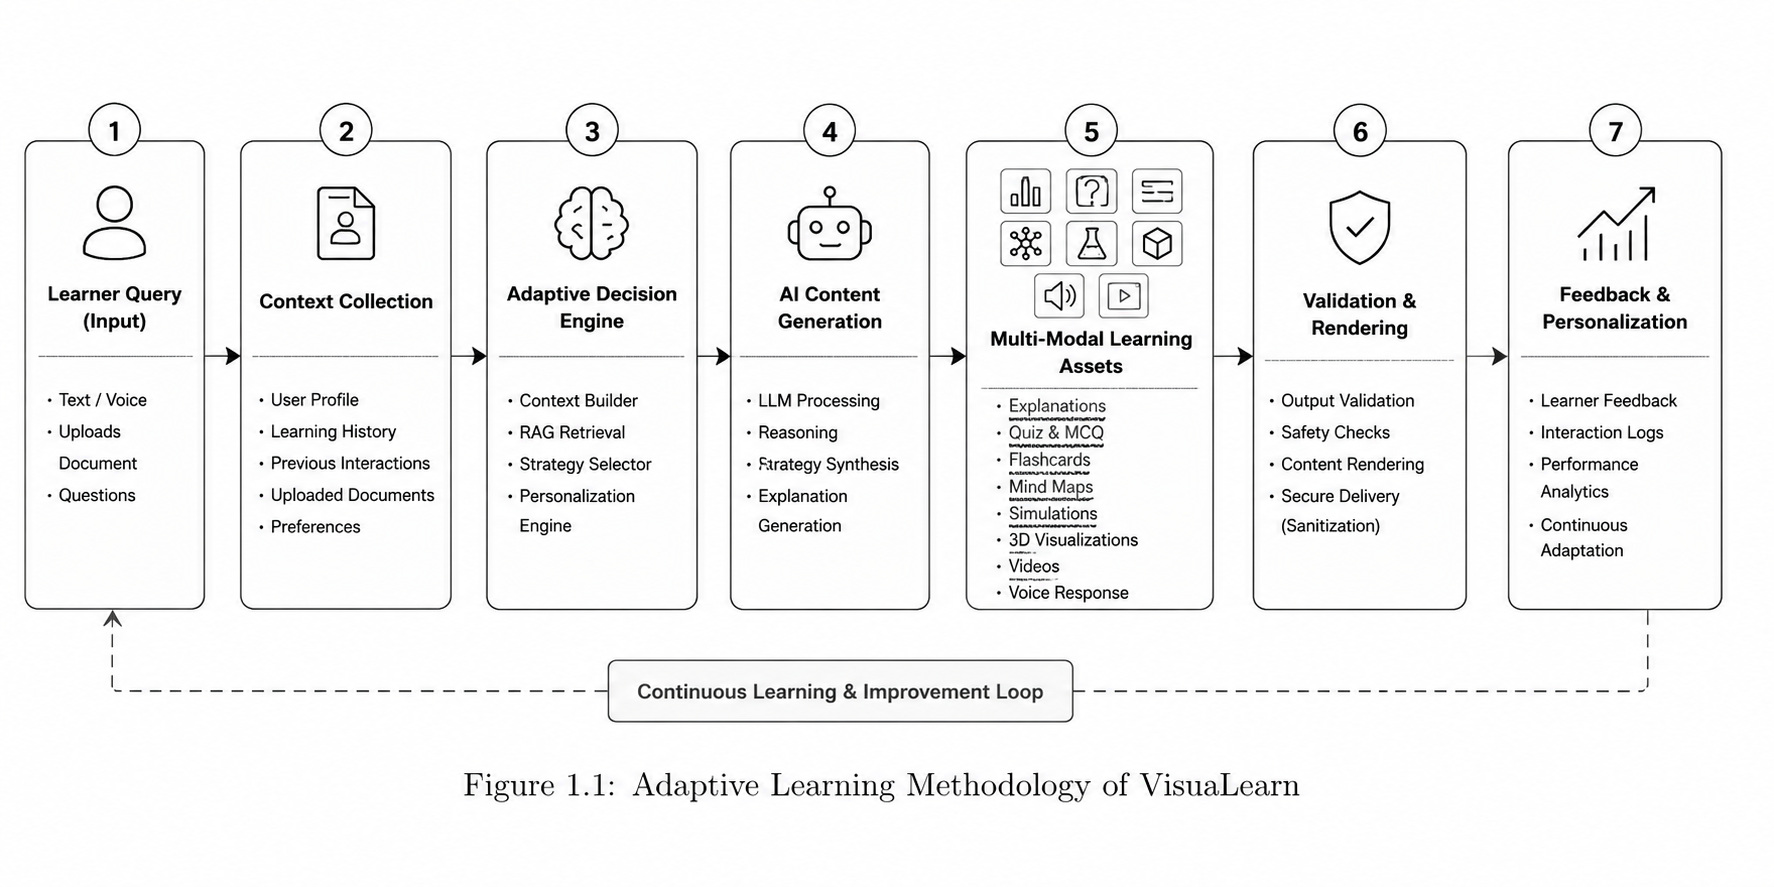
\includegraphics[width=0.95\textwidth]{Chapter1/1.1}
\caption{High-level methodology and adaptive learning workflow}
\label{fig:methodology}
\end{figure}

\section[Assumptions made / Constraints of the project]{\textbf{Assumptions made / Constraints of the project}}

The project assumes that users have internet access, a modern browser, and a valid Supabase login. The backend requires configured environment variables for Supabase and AI-provider services. Optional features such as text-to-speech, image generation, and real-time voice interaction depend on external provider support and browser permissions.

The main constraints are API cost, model latency, external service availability, browser performance for visual rendering, and the quality of generated learning material. The system includes validation and feedback mechanisms, but learners or teachers still need to review content used for high-stakes academic work.

The implemented platform was evaluated with 30 participants using learning modules such as simulations, visual explanations, document-based learning, quizzes, and revision artifacts. The feedback from this evaluation is used in the report to discuss usability, engagement, and learner perception.

		
		%Chapter 2
		\chapter{Fundamentals and Literature Survey}

The development of VisuaLearn is based on concepts from intelligent tutoring systems, adaptive learning, learner modelling, educational visualization, simulation-based learning, structured revision, and reliable full-stack software design. This chapter separates the theoretical fundamentals from the literature survey so that the project can be understood as both a software system and a research-motivated educational tool.

\section[Fundamentals]{\textbf{Fundamentals}}

\subsection[Intelligent Tutoring Systems]{\textbf{Intelligent Tutoring Systems}}

An Intelligent Tutoring System (ITS) is a software system that provides instruction, feedback, and support to learners. Such systems usually contain a domain model, a learner model, a tutoring model, and an interface model. The domain model represents subject knowledge. The learner model stores the student's current understanding. The tutoring model decides the instructional action. The interface model presents the response to the learner.

VisuaLearn follows the same educational principle but implements it in a modern web-based form. The domain content is generated dynamically for different topics. The learner model is represented using conversation history, resource history, quiz results, engagement signals, and adaptive context. The tutoring model selects teaching strategies such as visual explanation, guided steps, quiz mode, Socratic questioning, or remediation.

\subsection[Adaptive Learning]{\textbf{Adaptive Learning}}

Adaptive learning modifies instruction based on learner needs. A learner who answers correctly may be ready for a harder example, while a learner who repeatedly fails may need remediation. A learner who spends more time on a topic may need a slower explanation, and a learner who quickly completes content may prefer a concise response.

In this project, adaptation is performed at the response level. The system does not only decide what topic should come next; it also decides how the current topic should be taught. The adaptive layer uses context features such as cognitive state, engagement level, topic status, performance trend, confidence, topic difficulty, previous failures, and response time. These features help the system select a suitable teaching mode.

\subsection[Educational Visualization and Simulation]{\textbf{Educational Visualization and Simulation}}

Educational visualization represents abstract ideas using diagrams, charts, animations, and interactive components. It is useful when learners need to understand structure, movement, sequence, or relationships. In computer science, visual learning helps explain algorithms, data structures, recursion, memory, and state transitions.

Simulation-based learning is useful for processes that can be represented as a sequence of states. Sorting algorithms can be shown through comparisons and swaps. Graph traversal can be shown through visited nodes and queues. CPU scheduling can be shown through timelines and process queues. This supports active learning because the learner observes the process rather than only reading about it.

\subsection[Structured Revision]{\textbf{Structured Revision}}

Learning does not end with understanding an explanation. Students need revision and practice to retain concepts. Flashcards support recall. Quizzes support self-assessment. Mind maps support conceptual organization. Examples support transfer of learning to new situations. VisuaLearn generates these revision artifacts from the learning session so that a single query can lead to notes, examples, flashcards, quizzes, simulations, and saved resources.

\section[Literature Survey]{\textbf{Literature Survey}}

Bloom \cite{Bloom1984} showed that individualized tutoring can produce substantially stronger learning outcomes than conventional classroom-only instruction. The limitation of human tutoring is scalability: one-to-one tutoring is difficult to provide continuously to every learner. This motivates software systems that approximate personalized guidance.

VanLehn \cite{VanLehn2011} reviewed the relative effectiveness of human tutoring, intelligent tutoring systems, and other tutoring systems. The study showed that tutoring effectiveness depends on the granularity and quality of interaction. This is relevant to VisuaLearn because the platform attempts response-level adaptation rather than only course-level sequencing.

Ma et al. \cite{Ma2014} conducted a meta-analysis of intelligent tutoring systems and learning outcomes. Their work supports the claim that ITS-style personalization can improve learning when learner state is modeled. However, many ITS implementations are domain-specific and do not naturally support open-ended learner questions, generated visual artifacts, or multimodal revision resources.

Mayer \cite{Mayer2009} and Sweller \cite{Sweller1988} provide the theoretical foundation for combining verbal and visual explanation while controlling cognitive load. Their work is directly relevant to visual explanations, simulations, and step-by-step breakdowns. The limitation is that these theories do not by themselves define a deployable AI learning platform.

Kasneci et al. \cite{Kasneci2023} discuss opportunities and challenges of large language models in education. LLMs can generate flexible explanations and respond to natural-language questions, but educational systems must handle hallucination, over-reliance, feedback quality, and learner safety. VisuaLearn addresses this through backend orchestration, validation, feedback, and persistent learning history.

Recent AI-in-education reviews also emphasize that AI systems should support personalization, feedback, and responsible deployment rather than act as isolated answer generators \cite{Chen2020}. This supports the project goal of building an integrated learning platform with authentication, storage, adaptive routing, and safe rendering.

\section[Literature Comparison Table]{\textbf{Literature Comparison Table}}

\begin{longtable}{p{0.22\textwidth}p{0.13\textwidth}p{0.11\textwidth}p{0.10\textwidth}p{0.11\textwidth}p{0.13\textwidth}}
\caption{Comparison of Existing Work with VisuaLearn}\\
\toprule
\textbf{Existing Work} & \textbf{Adaptive} & \textbf{Visual} & \textbf{Sim.} & \textbf{Revision} & \textbf{Personal.}\\
\midrule
Bloom tutoring model \cite{Bloom1984} & Yes & No & No & Partial & High\\
Traditional ITS \cite{VanLehn2011,Ma2014} & Yes & Partial & Partial & Partial & Yes\\
Adaptive hypermedia \cite{Brusilovsky2007} & Yes & Partial & No & Partial & Yes\\
Multimedia learning systems \cite{Mayer2009} & No & Yes & Partial & No & No\\
LLM-based tutoring \cite{Kasneci2023} & Partial & Partial & No & Partial & Partial\\
VisuaLearn AI & Yes & Yes & Yes & Yes & Yes\\
\bottomrule
\end{longtable}

\section[Research Gap]{\textbf{Research Gap}}

Existing systems commonly focus on isolated educational tasks such as tutoring, quizzes, visualization, or content delivery. Very few systems integrate adaptive teaching, simulations, generated revision material, multimodal interaction, document-based learning, and learner-context modeling within a single environment. Additionally, limited attention has been given to safe rendering and persistence of dynamically generated educational artifacts.

The major gaps identified from the literature are:
\begin{itemize}[leftmargin=1.2cm]
\item Many systems provide explanations but do not generate a complete set of learning artifacts.
\item Visualization and simulation are often separate tools rather than part of the tutoring flow.
\item Revision content is usually manually created by the learner.
\item Learner context is not always used to decide the teaching format for each response.
\item Safe rendering of generated interactive learning content is not consistently addressed.
\item LLM-based learning tools often lack persistent learning history, structured evaluation, and adaptive feedback loops.
\end{itemize}

\section[Proposed Solution]{\textbf{Proposed Solution}}

VisuaLearn addresses the identified research gaps through a unified adaptive learning architecture that combines conversational AI, visualization, simulations, revision generation, learner modeling, document-based learning, feedback, and persistent learning history. Unlike systems that provide only a chatbot response or a separate visualization tool, the proposed system supports multiple teaching strategies and dynamically selects the most suitable learning mode based on learner context.

The platform also treats generated learning content as a managed artifact. Responses, visual widgets, simulations, quizzes, flashcards, and learning resources are stored with the learner session. This supports continuity, revision, and future adaptation. Safety mechanisms such as authentication, route protection, validation, fallback handling, and logging are included so that generated content can be used more reliably.

\section[Summary]{\textbf{Summary}}

The literature supports the value of personalized instruction, visual learning, adaptive feedback, and structured revision. However, the reviewed work also shows that many systems treat these capabilities separately. VisuaLearn is positioned as an integrated AI learning platform that brings these features into a single workflow and prepares the system for usability and learning-effectiveness evaluation.

		
		%Chapter 3
		\chapter{System Design}

VisuaLearn AI is designed as a layered and modular system. The design separates user interaction, request orchestration, intelligent decision-making, educational content generation, simulation, visualization, voice interaction, and data persistence. This chapter presents the architecture, module-wise design, data flow, database design, and adaptive learning workflow.

\section[System Architecture]{\textbf{System Architecture}}
The system follows a five-layer architecture: presentation layer, application layer, intelligence layer, service layer, and data layer. Each layer has a clear responsibility and communicates with adjacent layers.

\begin{figure}[H]
\centering
\resizebox{0.85\textwidth}{!}{%
\begin{tikzpicture}[
box/.style={draw, rounded corners, minimum width=7.4cm, minimum height=0.9cm, align=center},
arrow/.style={-{Latex[length=2mm]}, thick},
node distance=0.6cm
]
\node[box] (p) {Presentation Layer: Chat, Learning Workspace, Voice, Settings};
\node[box, below=of p] (a) {Application Layer: Routing, Authentication, Sessions, Validation};
\node[box, below=of a] (i) {Intelligence Layer: Context Builder, Strategy Selector, Personalization};
\node[box, below=of i] (s) {Service Layer: Learning Content, Simulation, Visualization, Voice};
\node[box, below=of s] (d) {Data Layer: Users, Conversations, Resources, Feedback};
\draw[arrow] (p) -- (a);
\draw[arrow] (a) -- (i);
\draw[arrow] (i) -- (s);
\draw[arrow] (s) -- (d);
\draw[arrow] (d.east) .. controls +(2,0) and +(2,0) .. (a.east);
\end{tikzpicture}
}
\caption{Layered Architecture of VisuaLearn AI}
\label{fig:layeredarchitecture}
\end{figure}

\section[Presentation Layer Design]{\textbf{Presentation Layer Design}}
The presentation layer is implemented as a responsive web application. It provides the learner with the following views:
\begin{itemize}[leftmargin=1.2cm]
	\item Chat interface for asking questions and receiving responses.
	\item Learning workspace for notes, examples, flashcards, quizzes, mind maps, and simulations.
	\item Simulation viewer with playback controls.
	\item Visual widget frame for dynamic learning artifacts.
	\item Voice interface for spoken learning sessions.
	\item Settings page for personalization and account configuration.
\end{itemize}

The learning workspace is designed to reduce clutter. Instead of showing all generated content in one long page, each artifact is placed in a suitable tab or panel. This supports focused reading and easier revision.

\section[Application Layer Design]{\textbf{Application Layer Design}}
The application layer receives frontend requests and routes them to the correct backend module. It performs authentication, request validation, trace logging, error handling, and response formatting. It also supports streaming output so that learners can see responses progressively.

The application layer contains routes for chat, learning content, simulations, visualizations, voice sessions, documents, personas, progress, and settings. This modular routing structure makes the project easier to maintain and test.

\section[Intelligence Layer Design]{\textbf{Intelligence Layer Design}}
The intelligence layer is responsible for adapting the teaching strategy. It builds a context vector from learner signals and selects one of the supported response modes. The context includes:
\begin{itemize}[leftmargin=1.2cm]
	\item Cognitive state
	\item Engagement level
	\item Topic status
	\item Performance trend
	\item Confidence
	\item Topic difficulty
	\item Previous failures
	\item Response time
\end{itemize}

The teaching strategies are visual learning, guided steps, quiz checking, concise explanation, Socratic questioning, and remediation. The selected strategy influences how the learning response is generated and displayed.

\section[Service Layer Design]{\textbf{Service Layer Design}}
The service layer contains the core educational modules. The learning content service generates structured notes, examples, quizzes, flashcards, and mind maps. The simulation service determines whether a topic is procedural and generates state transitions. The visualization service prepares visual or spatial content. The voice service supports real-time spoken interaction. The resource service stores and retrieves generated learning artifacts.

\section[Data Layer Design]{\textbf{Data Layer Design}}
The data layer stores all persistent learning information. The main data entities are:
\begin{itemize}[leftmargin=1.2cm]
	\item Users: authentication and profile details.
	\item Conversations: learning sessions created by users.
	\item Messages: learner queries and system responses.
	\item Learning resources: notes, quizzes, flashcards, mind maps, simulations, and visual references.
	\item Feedback records: quiz results, completion data, and learner ratings.
	\item Adaptive decisions: selected strategy, context, and reward information.
\end{itemize}

\section[Data Flow Diagram]{\textbf{Data Flow Diagram}}
\begin{figure}[H]
\centering
\resizebox{0.95\textwidth}{!}{%
\begin{tikzpicture}[
entity/.style={draw, rectangle, rounded corners, minimum width=2.8cm, minimum height=0.8cm, align=center},
process/.style={draw, ellipse, minimum width=3.0cm, minimum height=0.95cm, align=center},
store/.style={draw, cylinder, shape border rotate=90, aspect=0.28, minimum width=1.5cm, minimum height=1.1cm, align=center},
arrow/.style={-{Latex[length=2mm]}, thick},
node distance=0.9cm
]
\node[entity] (user) {Learner};
\node[process, right=of user] (request) {Request Processing};
\node[process, right=of request] (engine) {Learning Engine};
\node[entity, right=of engine] (output) {Learning Output};
\node[store, below=of request] (db) {Data Store};
\draw[arrow] (user) -- (request);
\draw[arrow] (request) -- (engine);
\draw[arrow] (engine) -- (output);
\draw[arrow] (request) -- (db);
\draw[arrow] (engine) -- (db);
\draw[arrow] (db) -- (request);
\end{tikzpicture}
}
\caption{Data Flow Diagram of VisuaLearn AI}
\label{fig:dataflow}
\end{figure}

\section[Adaptive Learning Workflow]{\textbf{Adaptive Learning Workflow}}
The adaptive workflow connects learner behavior with future teaching decisions. When a learner asks a question, the system builds context and selects a response strategy. After the learner interacts with the output, feedback is stored. The feedback affects future decisions.

\begin{figure}[H]
\centering
\resizebox{0.95\textwidth}{!}{%
\begin{tikzpicture}[
box/.style={draw, rounded corners, minimum width=2.6cm, minimum height=0.85cm, align=center},
arrow/.style={-{Latex[length=2mm]}, thick},
node distance=0.55cm
]
\node[box] (q) {Question};
\node[box, right=of q] (c) {Context};
\node[box, right=of c] (p) {Policy};
\node[box, right=of p] (r) {Response};
\node[box, right=of r] (f) {Feedback};
\draw[arrow] (q) -- (c);
\draw[arrow] (c) -- (p);
\draw[arrow] (p) -- (r);
\draw[arrow] (r) -- (f);
\draw[arrow] (f.south) .. controls +(0,-0.7) and +(0,-0.7) .. (c.south);
\end{tikzpicture}
}
\caption{Adaptive Learning Workflow}
\label{fig:adaptiveworkflow}
\end{figure}

\section[Module Interaction]{\textbf{Module Interaction}}
The modules interact in a sequential but flexible manner. A single learner query may produce a direct explanation, a learning resource, a simulation, a visual widget, or a voice response. The backend decides which module is suitable based on query intent and learner context. All generated resources are saved so that the frontend can reload them during future sessions.

\section[Design Summary]{\textbf{Design Summary}}
The design of VisuaLearn AI emphasizes modularity, adaptability, reliability, and usability. The layered architecture allows independent development of the frontend, backend, intelligent services, and data storage. The adaptive workflow supports personalization, while the learning workspace organizes outputs into meaningful educational artifacts.

		
		%Chapter 4
		\chapter{Implementation}

VisuaLearn AI was implemented as a full-stack learning platform in which the browser interface, API server, database layer, AI-service calls, and generated learning resources are kept as separate parts of the system. The implementation follows the design described in the previous chapter and converts it into working modules for conversation, structured learning material, simulations, visual content, voice interaction, feedback, and persistence.

\section[Development Environment]{\textbf{Development Environment}}
The frontend was developed with React and Vite. React was used to build reusable interface components, while Vite provided the local development server and production build pipeline. Tailwind CSS was used for styling, spacing, and responsive behaviour. Framer Motion was included only for limited interface transitions where movement helped the user understand a state change.

The backend was developed with Node.js and Express.js. Express route modules expose the application features through API endpoints, while middleware handles authentication, validation, rate control, and error handling. Supabase provides user authentication, PostgreSQL storage, and file storage. The source code is divided into separate frontend and backend folders so that interface changes, API logic, and database access can be maintained independently.

\section[Frontend Implementation]{\textbf{Frontend Implementation}}
The frontend is organised around pages, reusable components, and custom hooks. The main pages include the home page, authentication pages, chat page, learning page, dashboard, and settings page. Shared interface components include the sidebar, message list, message bubble, learning workspace, voice overlay, simulation viewer, widget frame, persona card, and feedback controls.

The chat page acts as the learner's starting point. A submitted question is sent to the backend, and the response is streamed back into the conversation view. Tool choices such as quiz, flashcard, mind map, simulation, or visualisation are represented in the input area before submission so that the learner can see what has been selected and remove it if needed.

The learning page displays generated resources in separate sections instead of placing every resource in one long output. Explanations, examples, flashcards, quizzes, mind maps, simulations, and visualisations are shown only when the corresponding section is opened or when the selected mode requires it. This layout reduces crowding on smaller screens and keeps the learner focused on the current activity.

Custom hooks are used for stateful frontend tasks. Chat streaming, authentication state, learning-resource loading, simulation state, voice recording, feedback submission, progress tracking, and stored-resource retrieval are handled outside the display components. This keeps the rendering components smaller and makes the behaviour easier to test and update.

\section[Backend Implementation]{\textbf{Backend Implementation}}
The backend is structured into route modules, middleware, service functions, agents, database clients, and utility functions. Each feature has a clear entry point through the API layer. Separate route modules handle chat, learning content, simulation, visualisation, voice sessions, document resources, personas, user progress, and stored learning resources.

Authentication middleware verifies the user before protected routes are executed. Request validation checks the shape of incoming data before it reaches the service layer. Rate limiting protects expensive endpoints, especially those that can call external AI services. Error handling middleware returns controlled error responses and prevents internal details from being exposed to the client.

The chat and learning endpoints support streamed responses. Streaming is used because generated educational answers may take several seconds, and the learner should be able to start reading while the remaining content is still being produced. Each generated response is linked to a conversation record so that the learner can reopen previous sessions and continue from stored context.

\section[Learning Content Implementation]{\textbf{Learning Content Implementation}}
The learning-content module converts a user question into structured study material. The output is not limited to a single explanatory paragraph. Depending on the request and the selected tool, the backend can prepare conceptual explanations, worked examples, analogies, flashcards, quiz questions, mind-map nodes, and summary blocks.

\begin{itemize}[leftmargin=1.2cm]
	\item Conceptual explanations
	\item Examples and analogies
	\item Flashcards
	\item Quiz questions
	\item Mind map nodes
	\item Summary blocks
\end{itemize}

Generated resources are normalised before they are returned to the frontend. Normalisation gives the interface predictable fields for titles, content blocks, choices, answers, nodes, and metadata. This avoids forcing the frontend to parse free-form text for every resource type.

Resource generation is also lazy where possible. For example, flashcards or quiz questions can be generated when the learner opens that section rather than during the first answer. Stored resources are reused when available, which reduces repeated calls to the backend and keeps later visits to the same conversation faster.

\section[Adaptive Learning Implementation]{\textbf{Adaptive Learning Implementation}}
The adaptive layer records learner signals and uses them to select a response strategy. The context vector includes cognitive state, engagement level, topic status, performance trend, confidence, topic difficulty, previous failures, and response time. These values are collected or derived before the next response is generated.

The supported teaching strategies are:
\begin{enumerate}[leftmargin=1.2cm]
	\item Visual learning for concepts that need diagrams or widgets.
	\item Guided steps for procedures and algorithms.
	\item Quiz mode for checking understanding.
	\item Concise explanation for short clarification.
	\item Socratic questioning for guided reflection.
	\item Remediation for correcting misconceptions.
\end{enumerate}

After a strategy is selected, the backend adds the corresponding instruction to the generation request. The generated answer is then checked for basic structural compliance. For example, a quiz response should contain a question, and a guided-step response should contain an ordered explanation. Feedback such as quiz correctness, completion, and engagement is recorded so that later response selection can use evidence from previous interactions.

\begin{figure}[H]
\centering
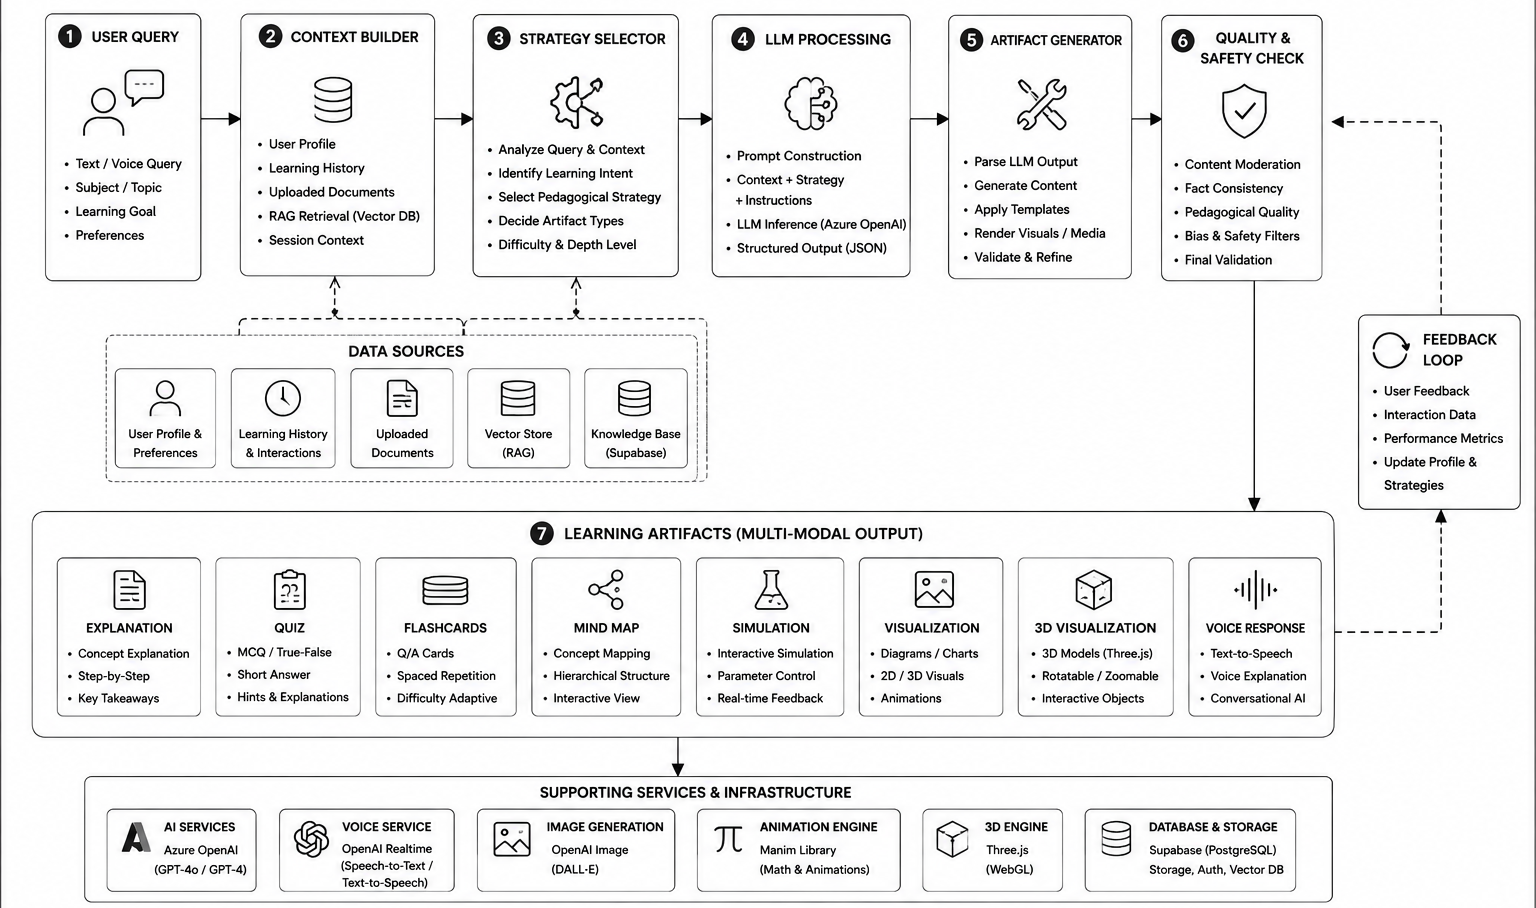
\includegraphics[width=0.92\textwidth]{Chapter4/some}
\caption{Adaptive strategy selection workflow}
\label{fig:adaptive-selection-strategy}
\end{figure}

\section[Simulation Implementation]{\textbf{Simulation Implementation}}
The simulation module first checks whether the requested topic can be represented as a sequence of observable states. Suitable topics include sorting algorithms, graph traversal, stacks, queues, heaps, linked lists, trees, state machines, grids, and timelines. When a topic is suitable, the backend prepares steps that describe how the state changes over time.

The frontend simulation viewer renders these steps with controls for play, pause, next, previous, and reset. The learner can inspect a single state or move through the process in order. In bubble sort, the viewer can show comparisons and swaps. In graph traversal, it can show the order in which nodes are visited. This stepwise display makes intermediate operations visible instead of presenting only the final answer.

\section[Visualization Implementation]{\textbf{Visualization Implementation}}
The visualisation module is used when a topic benefits from spatial, structural, or process-based representation. Before rendering, the system checks whether the generated visual content is safe and whether the device can support the required display. This prevents unsuitable visual output from affecting the rest of the application.

Generated visual widgets are displayed inside an isolated frame. The frame separates generated visual content from the main application interface. The content is validated and sanitised before display, and fallback messages are shown when rendering is not possible. This approach allows dynamic visual material to be used without giving generated content access to the main application state.

\section[Voice Interaction Implementation]{\textbf{Voice Interaction Implementation}}
The voice module allows a learner to ask questions through speech. The frontend records microphone input and connects it to a backend voice session. The backend associates the voice session with the learner context and the active conversation. Transcripts are written back into the chat flow so that spoken interactions remain part of the learning history.

Voice support is useful for short follow-up questions and revision sessions. It also improves access for learners who prefer speaking or who find typed interaction slower. The implementation keeps voice as an optional input path, so the normal text-based workflow remains available at all times.

\section[Persistence Implementation]{\textbf{Persistence Implementation}}
Persistence is implemented through Supabase. The database stores users, conversations, messages, learning resources, personas, feedback records, and adaptive decision records. Each generated learning resource is connected to a conversation. This allows the learner to reopen a previous session and access saved notes, flashcards, quizzes, mind maps, simulations, and visual resources.

The storage layer also reduces repeated generation. If a resource already exists for a conversation, the frontend can load it from storage instead of requesting a new generation. This improves response time and reduces unnecessary calls to external AI services.

\section[Deployment Architecture]{\textbf{Deployment Architecture}}
The deployment architecture separates the browser client, backend API, database services, storage, and external AI providers. The React client communicates with the Express backend through protected API routes. The backend performs authentication checks, request validation, learning orchestration, document retrieval, and AI-service calls. Supabase stores authenticated user data, conversations, generated learning resources, feedback records, and uploaded document metadata.

\begin{figure}[H]
\centering
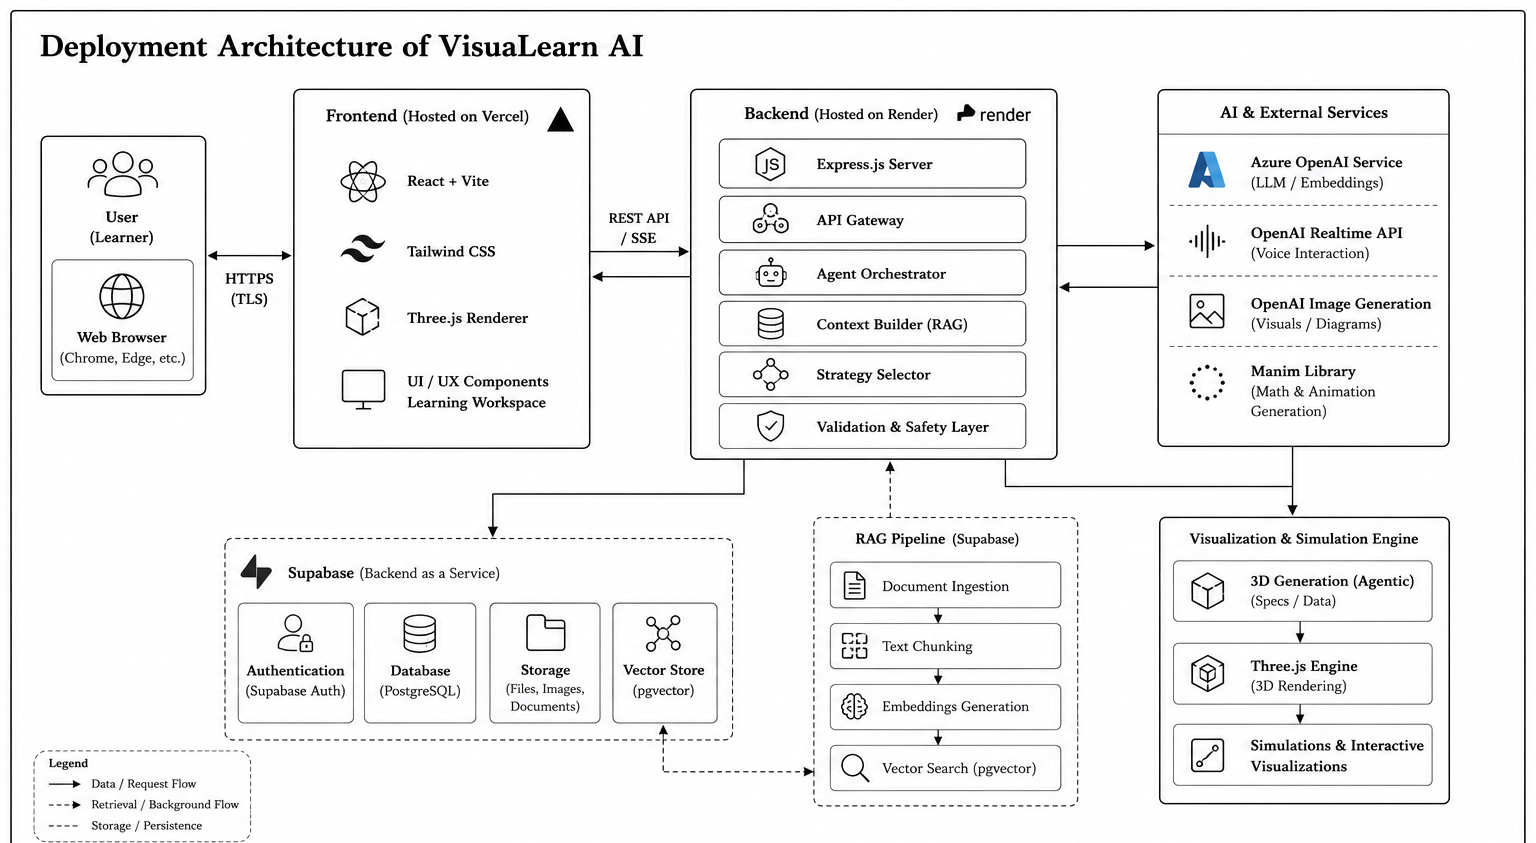
\includegraphics[width=0.92\textwidth]{Chapter4/dep}
\caption{Deployment architecture of VisuaLearn}
\label{fig:deployment-architecture}
\end{figure}

Provider keys and service credentials are kept on the server side. The browser sends requests to the backend rather than calling AI providers directly. This arrangement reduces credential exposure and allows backend routes, database storage, frontend hosting, and AI-service usage to be scaled or monitored separately.

\section[Security and Reliability Implementation]{\textbf{Security and Reliability Implementation}}
The implementation includes security and reliability measures at several points in the request flow:
\begin{itemize}[leftmargin=1.2cm]
	\item Protected routes for authenticated users.
	\item Request validation for malformed inputs.
	\item Rate limiting for controlled usage.
	\item Isolated rendering for generated visual artifacts.
	\item Fallback responses when a module fails.
	\item Structured logging for debugging and monitoring.
	\item Caching for repeated or expensive operations.
\end{itemize}

These measures are intended to keep failures local to the affected feature. For example, if a generated widget cannot be displayed, the chat and stored learning resources should still remain usable. Similarly, if a cached resource is available, the learner can continue studying even when a new generation request is delayed.

\section[Implementation Summary]{\textbf{Implementation Summary}}
The implementation delivers the main workflow required by VisuaLearn AI. A learner can ask questions, receive structured explanations, open revision resources, run simulations, view visual material, use voice input, submit feedback, and return to stored sessions. The modular structure keeps the main features separate while allowing them to operate together through shared conversation records, learner context, and stored resources.

		
		%Chapter 5
		\chapter{Testing and Results}

Testing was performed to verify that VisuaLearn AI satisfies its functional requirements, responds correctly to learner actions, stores learning resources, and remains usable across devices. The system contains several interacting modules, so testing was carried out at the frontend, backend, database, simulation, visualization, voice, and learning workflow levels.

\section[Testing Strategy]{\textbf{Testing Strategy}}
The testing strategy included the following:
\begin{itemize}[leftmargin=1.2cm]
	\item Functional testing of login, chat, learning resources, simulation, visualization, and settings.
	\item Backend route testing for valid and invalid requests.
	\item Manual testing of complete learner workflows.
	\item Simulation testing using deterministic algorithm examples.
	\item Responsive testing on desktop and mobile screen sizes.
	\item Error handling tests for missing input, unavailable resources, and rendering failures.
	\item Persistence testing for conversations, messages, and learning resources.
\end{itemize}

\section[Functional Test Cases]{\textbf{Functional Test Cases}}
\begin{longtable}{p{1.1cm}p{4cm}p{5.3cm}p{2.3cm}}
\caption{Functional Test Cases}\\
\toprule
\textbf{ID} & \textbf{Scenario} & \textbf{Expected Result} & \textbf{Status}\\
\midrule
TC01 & User login & Valid user is authenticated and redirected to the application & Passed\\
TC02 & New conversation & A new learning session is created and shown in recent sessions & Passed\\
TC03 & Ask question & The system returns an educational response and stores it & Passed\\
TC04 & Open learning workspace & Learning tabs and generated resources are displayed & Passed\\
TC05 & Generate flashcards & Flashcards appear with question and answer structure & Passed\\
TC06 & Generate quiz & Questions, options, and feedback are shown & Passed\\
TC07 & Generate mind map & Concepts are organized as related nodes & Passed\\
TC08 & Detect simulation topic & Suitable procedural topics open simulation workflow & Passed\\
TC09 & Invalid input & A controlled error or fallback response is shown & Passed\\
TC10 & Logout & User session is cleared securely & Passed\\
\bottomrule
\end{longtable}

\section[Learning Workflow Testing]{\textbf{Learning Workflow Testing}}
The learning workflow was tested using topics from computer science, grammar, general science, and engineering. Example queries included merge sort, breadth-first search, parts of speech, machine learning, neural networks, selection sort, and how an engine works. These topics were selected because they require different learning formats.

Algorithmic topics were suitable for simulations and guided steps. Conceptual topics were suitable for explanations, examples, flashcards, and quizzes. Grammar topics were suitable for examples and assessment. This confirmed that the system can organize learning support based on topic type.

\section[Simulation Testing]{\textbf{Simulation Testing}}
Simulation testing focused on state correctness. For sorting algorithms, the array state was checked after each comparison and swap. For graph traversal, the visited node order was inspected. For stack and queue topics, push, pop, enqueue, and dequeue operations were checked. For tree topics, node relationships and traversal order were verified.

The results showed that the simulation module works best for deterministic processes. For topics that do not have clear state transitions, the system avoids forcing simulation and instead provides structured explanations.

\section[Visualization Testing]{\textbf{Visualization Testing}}
Visualization testing verified whether generated visual components load safely and whether fallback messages appear when rendering is not possible. Device capability checks were used to avoid heavy visual rendering on unsupported devices. The isolated widget frame helped prevent invalid visual content from affecting the full application.

\section[Responsive Testing]{\textbf{Responsive Testing}}
The application was tested on desktop and mobile widths. The sidebar, chat input, learning content, flashcard cards, quiz view, simulation view, and settings page were checked for overflow and readability. Mobile improvements focused on keeping the main learning content visible, reducing unnecessary side content, and preventing persona or status labels from overflowing.

\section[Error Handling Testing]{\textbf{Error Handling Testing}}
Error handling was tested by submitting incomplete requests, unavailable resources, unsuitable simulation topics, and rendering failures. The system returned controlled messages instead of exposing raw internal details. Fallback content helped preserve the learning flow even when one feature could not complete.

\section[Observed Results]{\textbf{Observed Results}}
The implementation produced the following results:
\begin{itemize}[leftmargin=1.2cm]
	\item Learners can create and continue learning conversations.
	\item Structured learning resources are generated and displayed in separate views.
	\item Flashcards and quizzes support revision and self-assessment.
	\item Mind maps organize related concepts visually.
	\item Simulations support procedural understanding for algorithmic topics.
	\item Voice interaction supports natural question asking and accessibility.
	\item Persistent storage allows learners to revisit previous sessions.
	\item Adaptive strategy selection supports more personalized response formats.
\end{itemize}

\section[Result Summary]{\textbf{Result Summary}}
Testing confirmed that VisuaLearn AI functions as an integrated adaptive learning workspace. The system performs best when topics can be represented through structured explanation, practice, visualization, or simulation. The platform successfully demonstrates the project objective of moving beyond plain answer generation toward a reusable and interactive learning environment.

		
		%Chapter 6
		\chapter{Conclusion and Future Enhancements}

VisuaLearn AI was developed as an adaptive learning platform that brings conversation, structured study material, revision tools, simulations, visual content, voice input, learner profiles, and stored learning history into one application. The work was motivated by the limitation of text-only tutoring interfaces, where a learner may receive an answer but still need separate tools for practice, visual explanation, or later revision.

\section[Conclusion]{\textbf{Conclusion}}
The project shows how a learner query can be converted into several forms of learning support. A single topic can be presented as an explanation, examples, flashcards, quiz questions, mind-map content, simulation steps, or visual material depending on the selected mode and the nature of the topic. This gives the learner more than one way to revisit the same concept.

The frontend provides the chat interface, learning workspace, tool selection, resource views, simulation display, visual frame, feedback controls, and voice entry points. The backend coordinates authentication, conversation handling, learning-resource generation, adaptive strategy selection, simulation planning, visualisation handling, voice-session support, and database access. Supabase stores users, conversations, generated resources, feedback, personas, and decision records so that study material can be reopened after the original session.

The adaptive part of the system uses learner context and interaction signals to choose a response form. This makes the platform different from a fixed question-answer interface. The system can choose a visual response, guided steps, a quiz check, a concise explanation, Socratic questioning, or remediation based on the available context. The implementation therefore demonstrates a working link between learner state, response planning, generated study material, and stored feedback.

Overall, the project satisfies its main objective of building an integrated AI-assisted learning workspace. The current version is suitable as a functional prototype for personalised study support, especially for subjects where learners benefit from explanation, revision, and visual or procedural representation.

\section[Advantages]{\textbf{Advantages}}
The main advantages of the system are:
\begin{itemize}[leftmargin=1.2cm]
	\item It combines explanation, practice, revision, simulation, visualisation, and voice-based interaction in a single learning workflow.
	\item It stores conversations and generated resources, which allows learners to return to previous study sessions.
	\item It supports adaptive response strategies instead of using the same answer format for every learner query.
	\item It helps procedural and structural topics through simulations, diagrams, and visual widgets.
	\item It separates frontend components, backend routes, AI-service calls, and database operations, which makes the implementation easier to extend.
	\item It includes fallback handling, validation, isolated visual rendering, and protected routes to improve reliability during normal use.
\end{itemize}

\section[Limitations]{\textbf{Limitations}}
The present implementation has the following limitations:
\begin{itemize}[leftmargin=1.2cm]
	\item Generated explanations and quiz material may still require teacher review before use in graded or high-stakes academic settings.
	\item Rich visual and simulation features depend on browser performance, screen size, and device capability.
	\item Voice interaction depends on microphone permission, network quality, and transcription reliability.
	\item Personalisation needs enough learner activity before the stored signals can represent the learner accurately.
	\item Some abstract or opinion-based topics cannot be converted into useful simulations.
	\item The current evaluation is preliminary and does not replace a controlled study with delayed retention measurement.
\end{itemize}

\section[Future Enhancements]{\textbf{Future Enhancements}}
The system can be improved through the following extensions:
\begin{itemize}[leftmargin=1.2cm]
	\item Add subject-specific simulation generators for physics, mathematics, electronics, data structures, and engineering processes.
	\item Provide a teacher dashboard for reviewing learner progress, generated resources, feedback, and repeated difficulty areas.
	\item Add pre-test, post-test, and delayed-retention workflows for stronger learning-outcome measurement.
	\item Improve flashcard scheduling through spaced repetition based on learner performance.
	\item Support collaborative study sessions where learners can share selected resources and discuss a topic.
	\item Provide offline export for notes, flashcards, quiz results, and selected visual resources.
	\item Add more accessibility settings for font size, colour contrast, voice use, keyboard navigation, and reduced motion.
	\item Conduct a larger user study with varied subjects, longer usage periods, and human-reviewed scoring.
\end{itemize}

\section[Final Remarks]{\textbf{Final Remarks}}
VisuaLearn AI presents a working implementation of an adaptive learning workspace for personalised study. It connects software modules for conversation, resource generation, visual learning, simulation, feedback, and persistence into one system. Future work should focus on stronger evaluation, broader subject coverage, improved accessibility, and closer teacher involvement so that the platform can move from prototype use toward dependable academic support.

		
		%% Uncomment the following 2 commands to add Appendix chapters
		\appendix
		\chapter{Appendix}

\section{Appendix A: Important Source Code Excerpts}
This appendix lists selected implementation excerpts from important VisuaLearn AI features. The complete project contains additional route handlers, services, components, and configuration files; only representative code is included here to show the core implementation approach.

\subsection{Central API Route Registration}
The backend keeps feature routes modular and registers them from a central API module. This helps separate chat, learning content, documents, feedback, simulation, visualization, and Notion integration.

\begin{tcblisting}{listing only,colback=gray!10!white,breakable,boxsep=0pt,top=1mm,bottom=1mm,left=1mm,right=1mm,
listing options={basicstyle=\footnotesize\ttfamily,backgroundcolor=\color{gray!20},breaklines=true,columns=fullflexible}}
// backend/src/api/index.js
import express from 'express';
import learningContentRoutes from './learning/index.js';
import documentRoutes from './documents/routes.js';
import feedbackRoutes from './feedback/routes.js';
import simulationRoutes from './simulation/routes.js';
import visual3dRoutes from './visual3d/routes.js';
import notionRoutes from './notion/routes.js';
import chatRoutes from '../../routes/chat.js';

export function registerRoutes(app) {
  const router = express.Router();

  router.use('/learning-content', learningContentRoutes);
  router.use('/documents', documentRoutes);
  router.use('/feedback', feedbackRoutes);
  router.use('/simulation', simulationRoutes);
  router.use('/visual3d', visual3dRoutes);
  router.use('/notion', notionRoutes);
  router.use('/chat', chatRoutes);

  app.use('/api', router);
}
\end{tcblisting}

\subsection{Document Upload and RAG Preparation}
Uploaded PDFs are validated, stored, recorded in the database, and then processed into chunks for document-based learning.

\begin{tcblisting}{listing only,colback=gray!10!white,breakable,boxsep=0pt,top=1mm,bottom=1mm,left=1mm,right=1mm,
listing options={basicstyle=\footnotesize\ttfamily,backgroundcolor=\color{gray!20},breaklines=true,columns=fullflexible}}
// backend/src/api/documents/routes.js
router.post('/upload', upload.single('file'), async (req, res) => {
  const userId = req.user?.userId;
  if (!userId) return res.status(401).json({ error: 'Authentication required' });
  if (!req.file) return res.status(400).json({ error: 'No file provided' });

  const validation = validatePdf(req.file.buffer);
  if (!validation.valid) {
    return res.status(400).json({ error: validation.error });
  }

  const filename = `${uuidv4()}.pdf`;
  const storagePath = `${userId}/${filename}`;

  await supabase.storage.from('documents').upload(storagePath, req.file.buffer, {
    contentType: 'application/pdf',
    upsert: false,
  });

  const document = await createDocument(
    userId,
    filename,
    req.file.originalname,
    req.file.size,
    storagePath,
    req.file.mimetype
  );

  await processPdfBuffer(document.id, req.file.buffer);
  res.json({ success: true, documentId: document.id });
});
\end{tcblisting}

\subsection{Embedding Endpoint Builder}
The RAG service supports both a full Azure embeddings URL and a base endpoint. This makes the embedding configuration flexible while still routing requests through the backend.

\begin{tcblisting}{listing only,colback=gray!10!white,breakable,boxsep=0pt,top=1mm,bottom=1mm,left=1mm,right=1mm,
listing options={basicstyle=\footnotesize\ttfamily,backgroundcolor=\color{gray!20},breaklines=true,columns=fullflexible}}
// backend/src/services/rag/index.js
export function buildEmbeddingRequestUrl(endpoint, deployment, apiVersion) {
  if (!endpoint) return null;

  const parsed = new URL(endpoint.trim());

  if (
    parsed.pathname.includes('/openai/deployments/') &&
    parsed.pathname.endsWith('/embeddings')
  ) {
    if (!parsed.searchParams.has('api-version')) {
      parsed.searchParams.set('api-version', apiVersion);
    }
    return parsed.toString();
  }

  const basePath = parsed.pathname.replace(/\/+$/, '');
  parsed.pathname = `${basePath}/openai/deployments/${deployment}/embeddings`;
  parsed.search = '';
  parsed.searchParams.set('api-version', apiVersion);
  return parsed.toString();
}
\end{tcblisting}

\subsection{Simulation API}
Simulation requests are routed through detection and generation endpoints. The response returns a structured simulation payload instead of exposing arbitrary frontend code execution.

\begin{tcblisting}{listing only,colback=gray!10!white,breakable,boxsep=0pt,top=1mm,bottom=1mm,left=1mm,right=1mm,
listing options={basicstyle=\footnotesize\ttfamily,backgroundcolor=\color{gray!20},breaklines=true,columns=fullflexible}}
// backend/src/api/simulation/routes.js
router.post('/detect', rateLimitSimulation, async (req, res) => {
  const { query } = req.body;
  if (!query || typeof query !== 'string') {
    return res.status(400).json({ success: false, error: 'query is required' });
  }

  const decision = LearningOrchestratorDecision({
    query,
    mode: req.body.mode || 'chat',
    conversationState: req.body.conversationState || {},
    requestedArtifact: req.body.requestedArtifact || null,
  });

  const support = detectSandboxSimulationSupport(decision.activeTopic || query, {
    explicitQuery: query,
    requestedArtifact: req.body.requestedArtifact || null,
  });

  res.json({ success: true, supported: support.supported, decision, ...support });
});
\end{tcblisting}

\subsection{Lazy Learning Content Loading}
The frontend learning hook fetches only the requested learning tab. This prevents every artifact from being generated for every normal conversation message.

\begin{tcblisting}{listing only,colback=gray!10!white,breakable,boxsep=0pt,top=1mm,bottom=1mm,left=1mm,right=1mm,
listing options={basicstyle=\footnotesize\ttfamily,backgroundcolor=\color{gray!20},breaklines=true,columns=fullflexible}}
// frontend/src/hooks/useLearningContent.js
const fetchTabContent = useCallback(async (
  query,
  tabType,
  userId = null,
  accessToken = null,
  preferences = null,
  conversationId = null,
  documentId = null
) => {
  if (!query?.trim() || !tabType) return null;

  const headers = { 'Content-Type': 'application/json' };
  if (accessToken) headers.Authorization = `Bearer ${accessToken}`;

  const response = await fetch(`${API_BASE}/api/learning-content`, {
    method: 'POST',
    headers,
    body: JSON.stringify({
      query,
      userId,
      contentType: tabType,
      preferences,
      conversationId,
      documentId,
    }),
  });

  return parseJsonResponse(response, 'Learning content service unavailable.');
}, []);
\end{tcblisting}

\section{Glossary}
\begin{description}[leftmargin=3.2cm,style=nextline]
	\item[Learning Artifact] A generated resource such as notes, quiz, flashcards, mind map, simulation, or visualization.
	\item[Adaptive Strategy] The selected teaching format for a learner response.
	\item[RAG] Retrieval-augmented generation using uploaded document chunks.
	\item[Simulation] A step-by-step representation of a procedural topic.
	\item[Persistence] Storage of conversations and generated resources for future access.
\end{description}

\clearpage
\section{Appendix B: Selected System Screenshots}
This appendix includes selected screenshots from the implemented VisuaLearn AI application. The figures show the main user-facing workflows across chat, persona selection, learning content, quizzes, flashcards, mind maps, simulation, and 3D visualization.

\begin{figure}[H]
\centering
\includegraphics[width=0.96\textwidth]{Figures/normal.png}
\caption{Chat mode interface showing an active conversation with streamed assistant response, message history, and input controls.}
\label{fig:appendix-normal-chat-entry}
\end{figure}

\begin{figure}[H]
\centering
\includegraphics[width=0.96\textwidth]{Figures/chat.png}
\caption{New conversation screen showing the primary VisuaLearn AI entry point for starting a general learning or chat session.}
\label{fig:appendix-chat-mode}
\end{figure}

\begin{figure}[H]
\centering
\includegraphics[width=0.96\textwidth]{Figures/persona.png}
\caption{Persona selection interface used to choose the tutoring style that guides the assistant's tone and explanation approach.}
\label{fig:appendix-persona-selection}
\end{figure}

\begin{figure}[H]
\centering
\includegraphics[width=0.96\textwidth]{Figures/learn.png}
\caption{Learning mode screen presenting structured explanatory content for a selected topic inside the learning workspace.}
\label{fig:appendix-learn-mode}
\end{figure}

\begin{figure}[H]
\centering
\includegraphics[width=0.96\textwidth]{Figures/quiz.png}
\caption{Quiz view generated for a learning topic, allowing the learner to test understanding through interactive questions.}
\label{fig:appendix-quiz-view}
\end{figure}

\begin{figure}[H]
\centering
\includegraphics[width=0.96\textwidth]{Figures/flashcards.png}
\caption{Flashcards view showing concise question-and-answer cards for revision and repeated practice.}
\label{fig:appendix-flashcards-view}
\end{figure}

\begin{figure}[H]
\centering
\includegraphics[width=0.96\textwidth]{Figures/mindmaps.png}
\caption{Mind map view organizing the selected topic into connected concepts for visual exploration.}
\label{fig:appendix-mindmap-view}
\end{figure}

\begin{figure}[H]
\centering
\includegraphics[width=0.96\textwidth]{Figures/sim.png}
\caption{Simulation view showing an interactive step-by-step representation of a learning concept.}
\label{fig:appendix-simulation-view}
\end{figure}

\begin{figure}[H]
\centering
\includegraphics[width=0.96\textwidth]{Figures/3d.png}
\caption{3D visualization view demonstrating an interactive spatial representation generated for a learning concept.}
\label{fig:appendix-3d-visualization}
\end{figure}
%Appendix Chapter 1
		
		\backmatter
		\ifDrf
		\else
		\clearpage
		\addcontentsline{toc}{chapter}{Bibliography}
		\printbibliography%
		\fi
	\end{spacing}
\end{document}
